\documentclass{homework}

\title{Thesis Outline}
\author{Kevin Evans}
\studentid{11571810}
\date{September 20, 2021}
\setclass{Physics}{490}

\usepackage{graphicx}
\usepackage{physics}
\usepackage{times}
\usepackage{hyperref}

\begin{document}
	\maketitle
	
	\section*{Abstract}
	\begin{itemize}
		\item Purpose: measure how chaotic the GPE is in 1D
		\item Methods: created Python simulations, modeled the GPE and calculated Lyapunov exponents as it evolves in time
		\item Results: the GPE has positive Lyapunov exponents in 1D. There seems to be a dependence on the energy of the system with the exponent
		\item Conclusion: further testing is needed to see how chaos arises, and how chaos is characterized in higher dimensions
	\end{itemize}
	
	\section{Introduction}
	\begin{itemize}

		
		\item Bose-Einstein condensates (BECs) are formed by bosonic gases (at low densities) are cooled near absolute zero, resulting in occupation of the lowest quantum state leading to various quantum effects
		\item The GPE is a nonlinear Schr\"odinger equation that models Bose Einstein condensates. If we used the Schr\"odinger equation directly, each equation would have to include a term for interaction, leading to a system of $O(N^2)$ equations. The GPE is instead a multiparticle wavefunction, which uses a mean-field (Hartree-Fock) approximation.
		
		\item Chaos is the exponential separation in distance and is characterized by positive Lyapunov exponents. Instead of using a Euclidian distance, we can find a new distance function for separation in Hilbert space (the realm of these wavefunctions)
		
		\item It is unclear how chaos arises in classical physics, considering that quantum physics (by the Schr\"odinger equation) is fundamentally linear (and linearity cannot lead to a positive Lyapunov exponent [need to find a citation]). 
		
	\end{itemize}
	
	\section{Background} 
	\begin{itemize}
		\item BECs are modeled by the GPE, which is a Hartree-Fock approximation---basically treating particle interaction as a mean-field---resulting in the $g$ term below
		
		\item The GPE is a nonlinear Schrodinger equation, \begin{align*}
			i \hbar \pdv{\Psi(\bvec{r}, t)}{t} & = \left(
			-\frac{\hbar^2}{2m} \laplacian + V(\bvec{r}) + g\abs{\Psi}^2
			\right) \Psi
		\end{align*}
		where the $g$-term is the coupling constant describing particle interaction. Positive $g$ is from repulsive interactions, which is what you'd expect in an actual BEC
		
		\item We can see how the PDE evolves in time by discretizing space and using a solver (like Runge-Kutta) to evolve it in time
		
		\item Lyapunov exponents characterize chaos \begin{itemize}
			\item Lorenz system is a classic example with positive exponents
			\item The trajectories of 3 planets can be considered chaotic
			\item The Lyapunov exponent $\lambda$ is defined for a separation vector $\bvec{Z}$ as 
			$$\abs{\delta \bvec{Z}(t)} \approx e^{\lambda t} \abs{\delta \bvec{Z}_0}.$$
			
			\item In the GPE, we're looking at the multiparticle wavefunction and we can look at ``differences'' in trajectories in different ways (differences in phase or amplitudes, etc.)
			\item Since wavefunctions exist in $L^2$, we need to find a new distance function instead of Euclidian distances. In Hilbert space, we can define a difference function as $$d^{(2)}(\psi_1, \psi_2, t) = \frac{1}{2} \braket{\psi_1 - \psi_2}{\psi_1 - \psi_2}.$$
		\end{itemize}
		
		\item Turbulence is hard to define, but we can see turbulence by looking at the energy vs $k$ plot and searching for a $-5/3$-power dissipation (``energy cascade'')
		\item There are also several potential sources of error that can lead to false positive exponents, like floating point and rounding errors, as well as errors in the Taylor expansion of functions
		
		\item Python is an easy-to-use and performant language for modeling physical phenomena. Can use libraries like numpy and scipy to evolve the GPE in time
	\end{itemize}
	
	\section{Procedures}
	\begin{itemize}
		\item Simulations were creating using Python with Numpy
		\item The GPE was approximated using a finite (spatial) difference technique initially
		\item Also used spectral methods
		\item An initial state $\psi_0$ was generated by imprinting turbulence and allowing the wavefunction to evolve in time. 
		\item Used an adaptive Runge-Kutta via \texttt{solve\_ivp} to evolve the wavefunction in time
		\item Separately, wrote a program showing linearity between \texttt{solve\_ivp} parameters and the Lyapunov exponent for the linear ($g=0$), showing tolerances of $10^{-12}$ is enough
	\end{itemize}
	
	\section{Findings}
	\begin{itemize}
		\item Positive Lyapunov exponents were found in the case of 1D
		\item Turbulent BECs are chaotic, where the BECs are imprinted with a random phase
		\item The Lyapunov exponent is proportional to the coupling constant of the GPE (for $g>0$):
		
		\begin{center}
			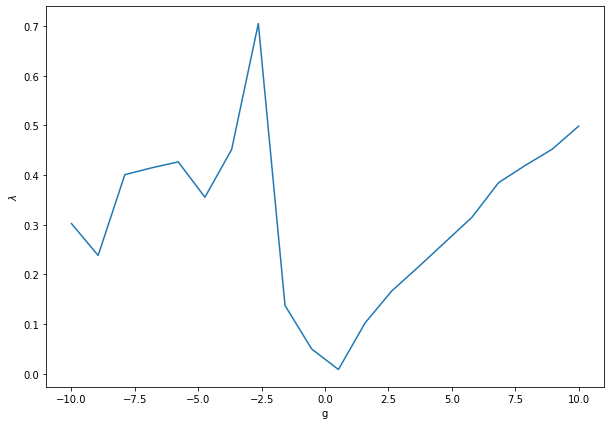
\includegraphics[width=0.7\linewidth]{g_vs_exp}
		\end{center}
		
		\item BECs with more vorticies seem to be less chaotic? Need to talk more with my advisor about this
	\end{itemize}
	
	\section{Summary and Conclusions} 
	\begin{itemize}
		\item The GPE exhibits chaos for $g>0$, with Lyapunov exponents proportional to $g$
		\item Likely not due to floating point or \texttt{solve\_ivp} atol/rtol errors
		\item Further testing is needed to see if chaos can be shown in higher dimensions (or perhaps this is just an artifact of 1D)
	\end{itemize}
	\section*{Appendices}
	\begin{itemize}
		\item Code samples?
		\item Could include additional plots
	\end{itemize}
	
	\section*{References}
	Essential ones:
	\begin{itemize}
		\item \href{https://journals.aps.org/prl/abstract/10.1103/PhysRevLett.62.2065}{https://journals.aps.org/prl/abstract/10.1103/PhysRevLett.62.2065}
		\item \href{https://journals.aps.org/pra/abstract/10.1103/PhysRevA.83.043611}{https://journals.aps.org/pra/abstract/10.1103/PhysRevA.83.043611}
		\item \href{https://journals.aps.org/prl/abstract/10.1103/PhysRevLett.71.2683}{https://journals.aps.org/prl/abstract/10.1103/PhysRevLett.71.2683}
		\item \href{https://arxiv.org/pdf/1605.09580.pdf}{https://arxiv.org/pdf/1605.09580.pdf}
		\item Pethick/Smith
	\end{itemize}
\end{document}